\begin{figure*}[!t]
\centering
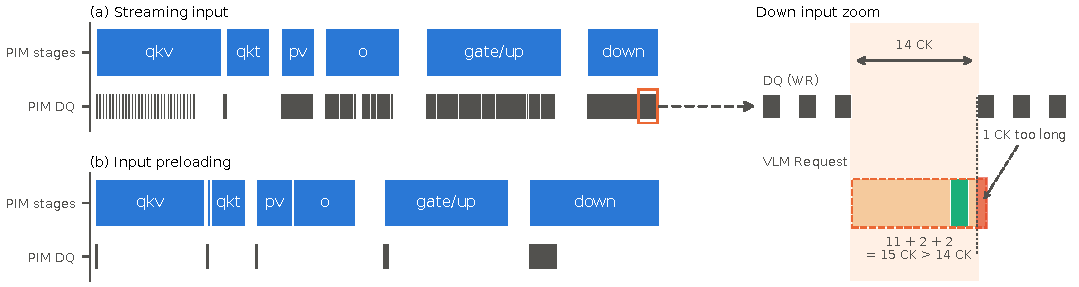
\includegraphics[width=\textwidth]{figures/fig7_step_timeline.pdf}
\setcounter{figure}{6}
\caption{第 0 个去噪步第 0 层的执行时间线（物理通道 0）。(a) 流式供数：PIM 的 DQ 突发散布在 QKV、O、Gate/Up、Down 的整个计算过程中。(b) 输入预装载（VLA-PIM）：PIM 的 DQ 传输集中在 7 个 I/O epoch（灰色）内，其余时间 DQ 全部归 GPU；VLM kernel 跨越多个 PIM 阶段连续执行，AE 的非线性算子只在阶段边界插入。}\label{fig:timeline}
\end{figure*}
